% 2020 全国Ⅰ卷 文19：圆锥（顶点 D，圆心 O，△ABC 内接正三角形，P 在 DO 上，∠APC=90°）
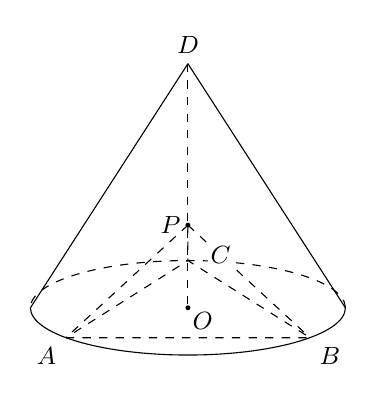
\begin{tikzpicture}[scale=1.0, font=\small]
  \coordinate (D) at (0,3.1);
  \coordinate (O) at (0,0);
  \coordinate (A) at (-1.55,-0.38);
  \coordinate (B) at (1.55,-0.38);
  \coordinate (C) at (0,0.6);
  \coordinate (P) at (0,1.05);
  \draw (-2,0) arc (180:360:2 and 0.6);
  \draw[dashed] (2,0) arc (0:180:2 and 0.6);
  \draw (D) -- (-2,0);
  \draw (D) -- (2,0);
  \draw[dashed] (D) -- (O);
  \draw[dashed] (A) -- (B) -- (C) -- cycle;
  \draw[dashed] (P) -- (A)  (P) -- (B)  (P) -- (C);
  \fill (O) circle (0.9pt);  \fill (P) circle (0.9pt);
  \node[above] at (D) {$D$};
  \node[below left] at (A) {$A$};
  \node[below right] at (B) {$B$};
  \node[right, xshift=7pt, yshift=2pt, fill=white, inner sep=1pt] at (C) {$C$};
  \node[below right, inner sep=1.5pt] at (O) {$O$};
  \node[left, inner sep=2.5pt] at (P) {$P$};
\end{tikzpicture}
